\documentclass[border=5pt]{standalone}
\usepackage{tikz}
\usepackage{amsmath,amssymb,bm}
\usetikzlibrary{arrows.meta, decorations.pathreplacing}

\begin{document}
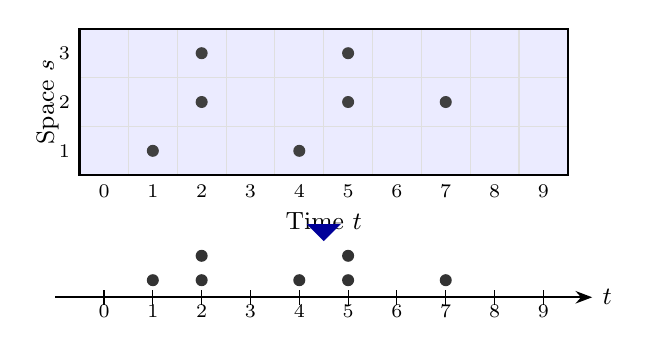
\begin{tikzpicture}[scale=0.62, every node/.style={font=\small}]

% ===== TOP: 2D Grid (s=1,2,3 only) =====

% Spatial window band (fills entire visible grid)
\fill[blue!8] (0,0) rectangle (10,3);

% Grid
\draw[gray!25, thin] (0,0) grid[step=1] (10,3);
\draw[thick] (0,0) rectangle (10,3);

% Axis labels
\node[below=10pt] at (5, 0) {Time $t$};
\node[rotate=90, above=4pt] at (0, 1.5) {Space $s$};
\foreach \x in {0,...,9}
  \node[below, font=\scriptsize] at (\x+0.5, 0) {\x};
\foreach \y/\lab in {0/1, 1/2, 2/3}
  \node[left, font=\scriptsize] at (0, \y+0.5) {\lab};

% Pattern P occurrences (s=1→y=0, s=2→y=1, s=3→y=2)
\foreach \t/\s in {
  1/0, 2/1, 2/2, 4/0, 5/1, 5/2, 7/1
}{
  \fill[black!75] (\t+0.5, \s+0.5) circle (3.5pt);
}

% ===== TRIANGLE (replaces arrow) =====
\fill[blue!60!black] (4.65, -1.0) -- (5.35, -1.0) -- (5, -1.35) -- cycle;

% ===== BOTTOM: 1D Timeline =====

% Timeline
\draw[thick, -{Stealth[length=6pt]}] (-0.5, -2.5) -- (10.5, -2.5)
  node[right, font=\small] {$t$};
\foreach \x in {0,...,9}
  \draw (\x+0.5, -2.65) -- (\x+0.5, -2.35)
    node[below=2pt, font=\scriptsize] {\x};

% Events on timeline (all black)
% Single occurrences
\fill[black!80] (1.5, -2.15) circle (3.5pt);  % t=1
\fill[black!80] (4.5, -2.15) circle (3.5pt);  % t=4
\fill[black!80] (7.5, -2.15) circle (3.5pt);  % t=7

% Duplicate at t=2 (stacked)
\fill[black!80] (2.5, -2.15) circle (3.5pt);   % t=2 (1st)
\fill[black!80] (2.5, -1.65) circle (3.5pt);   % t=2 (2nd)

% Duplicate at t=5 (stacked)
\fill[black!80] (5.5, -2.15) circle (3.5pt);   % t=5 (1st)
\fill[black!80] (5.5, -1.65) circle (3.5pt);   % t=5 (2nd)

\end{tikzpicture}
\end{document}
